\section*{Numerical treatment of the initial interface}


\section*{Theoretical vs simulated reflection coefficients}


\hl{NOTE TO SELF: FIX FLIPPING OF REFLECTION AND TRANSMISSION COEFFICIENT IN TEXT HERE}

\begin{align*}
  \boldsymbol{R}_{theoretical}=p_R/p_I=(-p_{reflected}+p_{atm})/(p_a-p_{atm})=((69.15+101325/p_{scale})/(71.42-0.714285714285714))=0.988
\end{align*}

To ensure that the numerical implementation of the interface is sufficiently sharp as to reflect the dynamics of a discontinuous interface, the simulated acoustic reflection coefficient $\boldsymbol{T}_S$ was calculated for the case of the $10$ MPa trapezoidal wave for varying thickness parameter delta $\delta$ and compared to the theoretical acoustic reflection coefficient $\boldsymbol{T}$, where 

\begin{align*}
  \boldsymbol{T}=\frac{2\left(\rho c\right)_{air}}{\left(\rho c\right)_{air}+\left(\rho c\right)_{water}}
\end{align*}


The prescribed interface thickness parameter (typically $\delta = 0.08\lambda$) was used to determine the initial volume fraction and density condition where the a distance parameter from the interface is defined as 
\begin{align*}
  d = \frac{\delta +y(x)_{interface} -y}{2\delta}.
\end{align*}
and the initial Volume fraction is written as 
\begin{align*}
  y_0 = %
  \begin{cases}
    1,\\%
    exp\left(log\left(10^{-16}\right)\abs{d}^8\right),\\%
    0,%
  \end{cases}%
\end{align*}

such that $d$ is normalized within the mixed air-water region.

\begin{figure}
\centering
  \centering
  \includegraphics[width=\textwidth]{./figs/lung_figs/p_snapshots}
  \caption{Snapshots of pressure throughout the waves time in the
    domain and shortly thereafter at $t=0, 3, 6, 9, 12, 25,$ and
    $30$. We observe that once the wave leaves the domain at
    approximately $t=21$ noticeable reflections do not occur.}
\end{figure}

\begin{figure}
\centering
%\begin{subfigure}{0.5\textwidth}
  \centering
  \includegraphics[width=0.5\textwidth]{./figs/lung_figs/delta_R}
%\end{subfigure}
  \caption{The reflection coefficient $\boldsymbol{R}$ based on
    calculated wave amplitudes is shown for various values of the
    interface thickness parameter $\delta = 0.01, 0.04, 0.08,$ and
    $0.16$. The default value for results in chapters
    \ref{ch:usbe_lung} and \ref{ch:usbe_lung_bio} is $\delta=0.08$ and
    indicated in red. The computed reflection coefficient appears to
    be approximately constant at $\boldsymbol{R}_{computed}=0.991$ for
    the range of interface thicknesses considered here. This is
    $0.3\%$ greater than the theoretical reflection
    coefficient $\boldsymbol{R}_{theoretical}=0.988$.}
\end{figure}


\begin{figure}
  \centering
  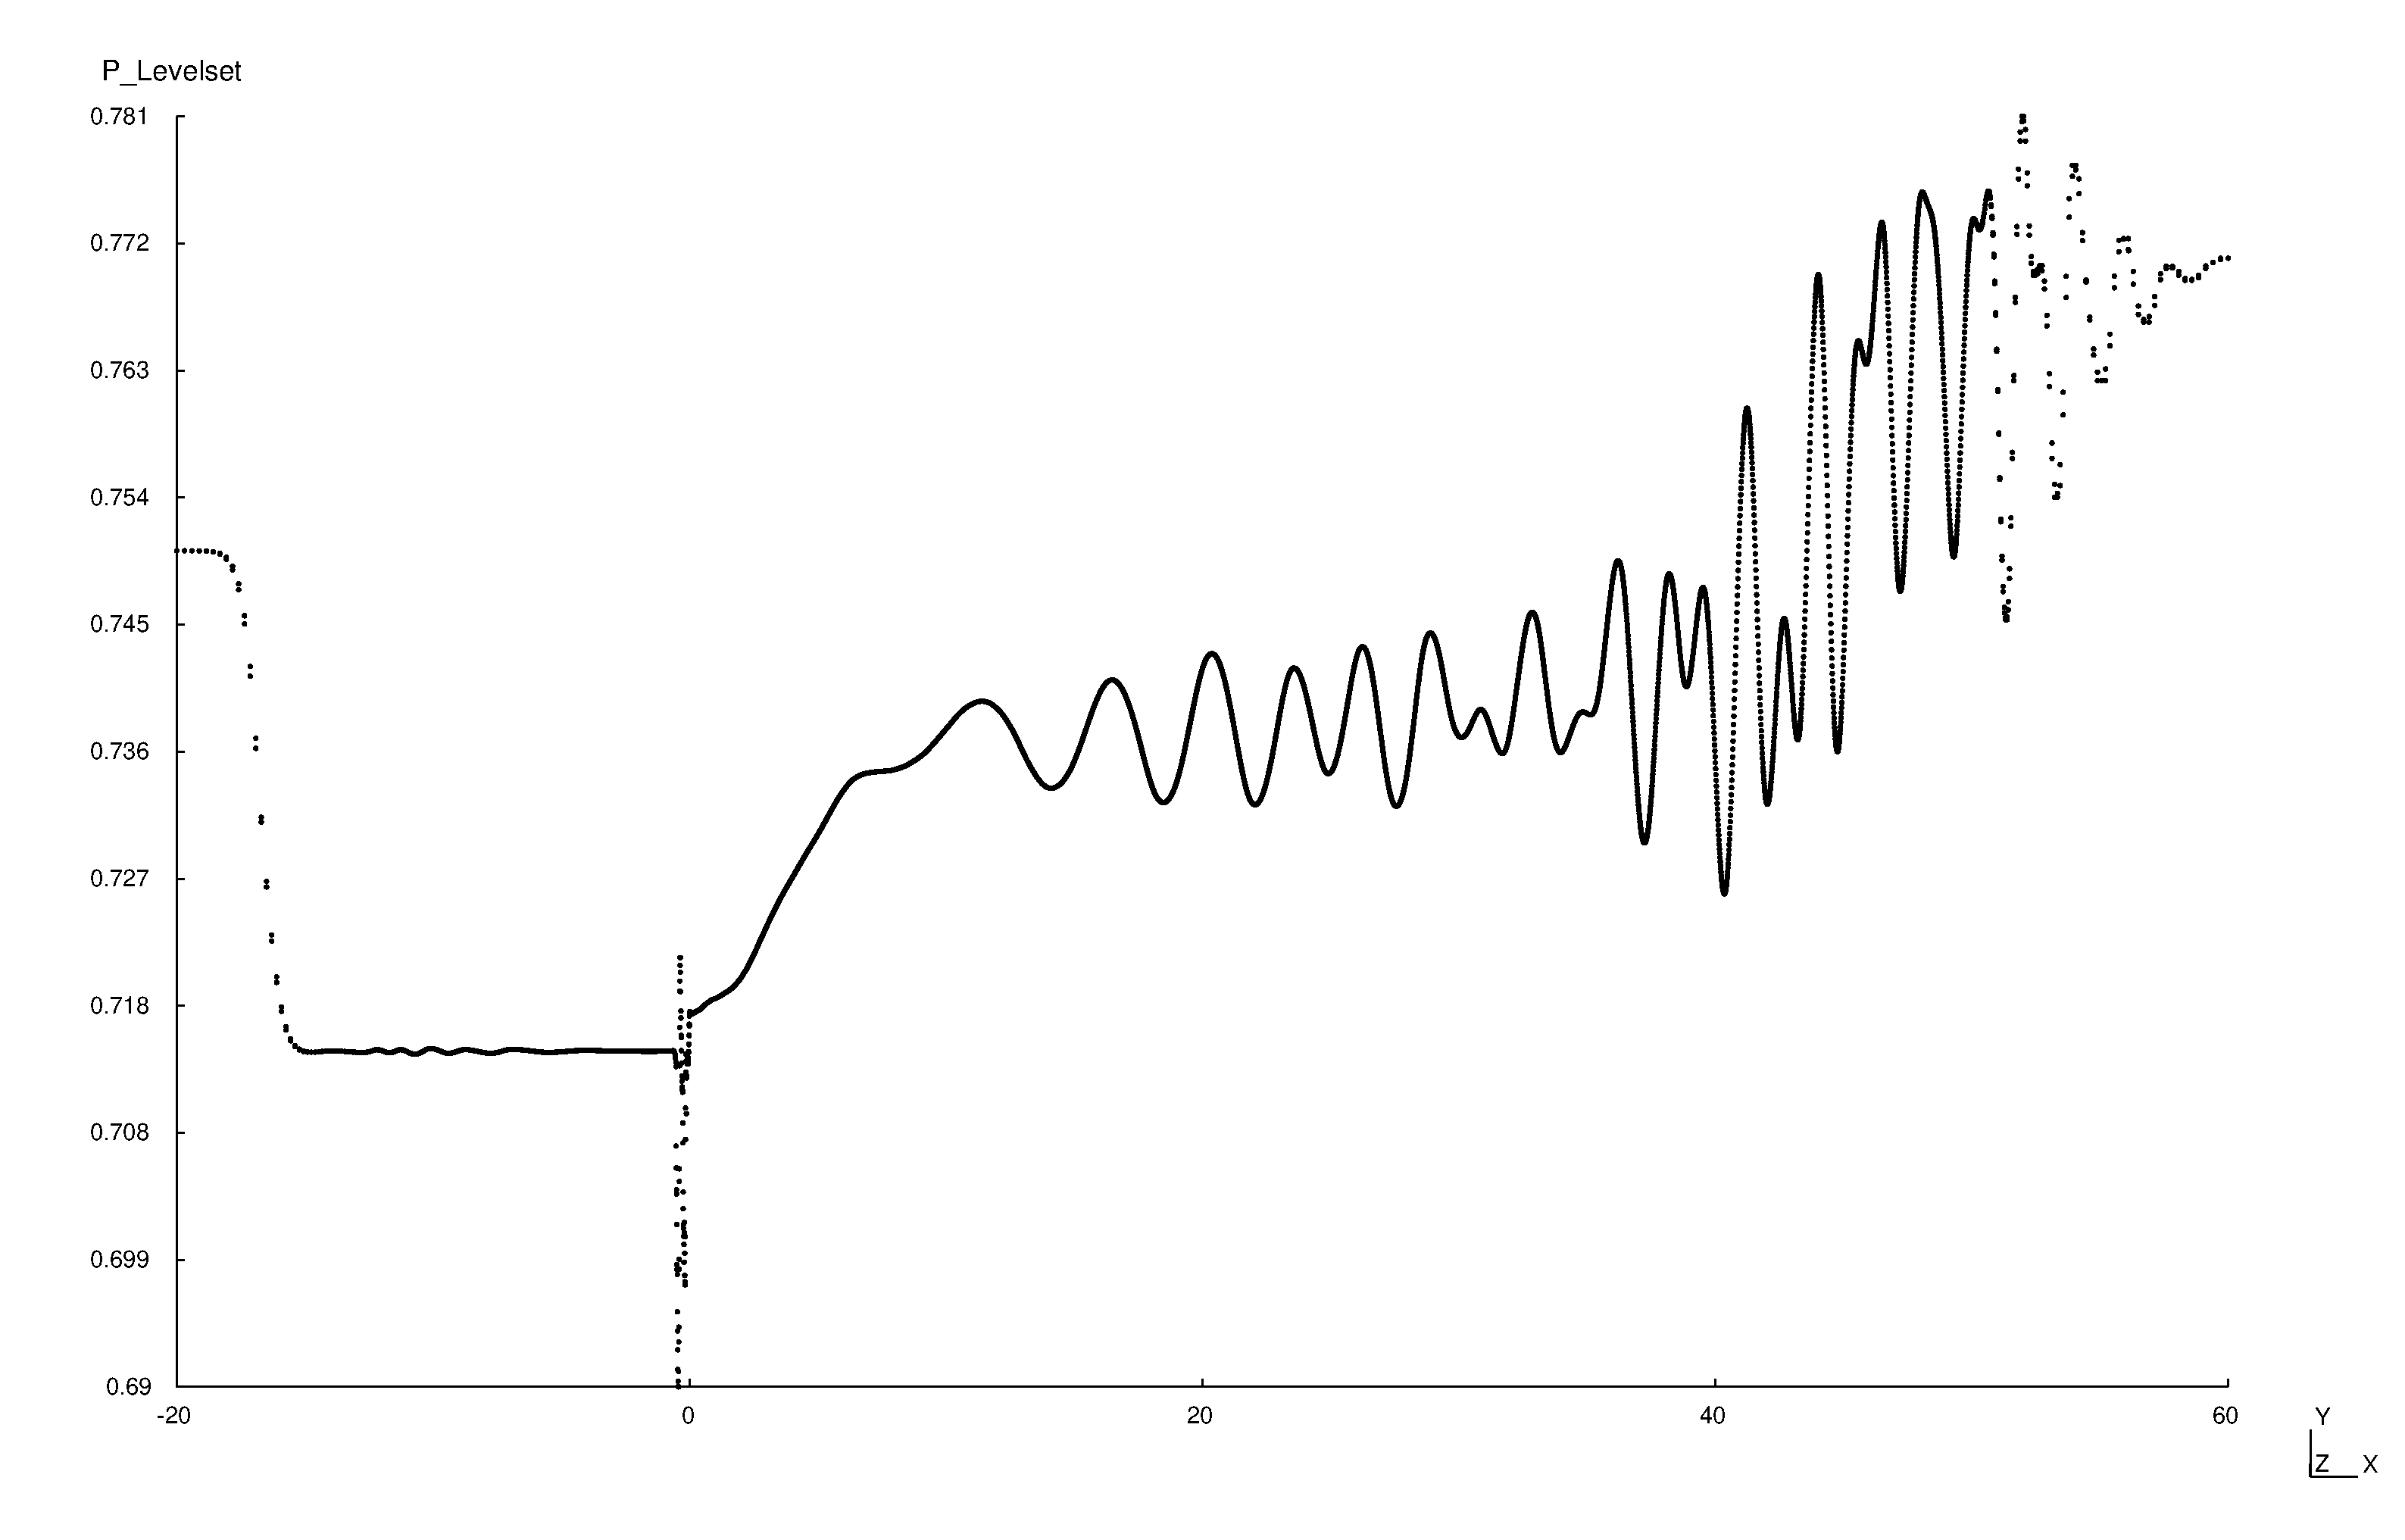
\includegraphics[width=\textwidth]{./figs/lung_figs/p_centerline_t25}
  \caption{Center-line pressure at t=25. At maximum, 0.1\% of the wave
    is artificially reflected back into the domain.}
\end{figure}


%%% Local Variables:
%%% mode: latex
%%% TeX-master: t
%%% End:
